
Notre projet de fin d'étude peut être séparé en deux parties distinctes:
\begin{itemize}
    \item Avant le passage en XL 
    \item Durant la période XL
\end{itemize}

\section{Avant le passage en XL}
Le projet a débuté avec plusieurs objectifs 
\subsection{Objectif SMART}
Afin de mieux délimiter le projet et ses objectifs, nous avons convenus avec le client d'un certain nombre d'objectifs, correspondant aux critères SMART (Spécifique, Mesurable, Atteignable, Réaliste et Temporairement défini).

Ces objectifs nous ont permis d'évaluer la charge de travail nécessaire à la réalisation du projet ainsi que de commencer a prévoir l'organisation générale.
Ils nous permettent également de pouvoir quantifier l'avancement du projet.

Ces objectifs sont: 
\begin{itemize}
    \item Construire un système d'extraction du texte brut depuis des PDF  
    \item Extraire une liste de métadonnées (définie avec le client) depuis le texte
    \item Assigner au moins une taxonomie au texte 
    \item Indexer les documents de notre base de données à partir des informations extraites (métadonnées et taxonomies)
    \item Réaliser une interface de sous la forme d'un moteur de recherche  
\end{itemize}

Pour être capables de vérifier si chacun de ces objectifs est atteint, nous avons mis en place une série de test, définie section~\ref{tests} du DER\@. 



\subsection{Gantt}
Dans un premier temps, nous avions réalisé un planning de Gantt avec les tâches principales.
Ce Gantt nous permet de faire une estimation de la charge de travail et la durée du projet. 

Avec la complexité du projet, nous avons décidé nous consacrer sur les tâches les plus importantes, c'est a dire les fonctionnalités d'extractions de données.
Le moteur de recherche et surtout son interface ont été classés comme secondaires pour le projet.

\begin{figure}[h!]
  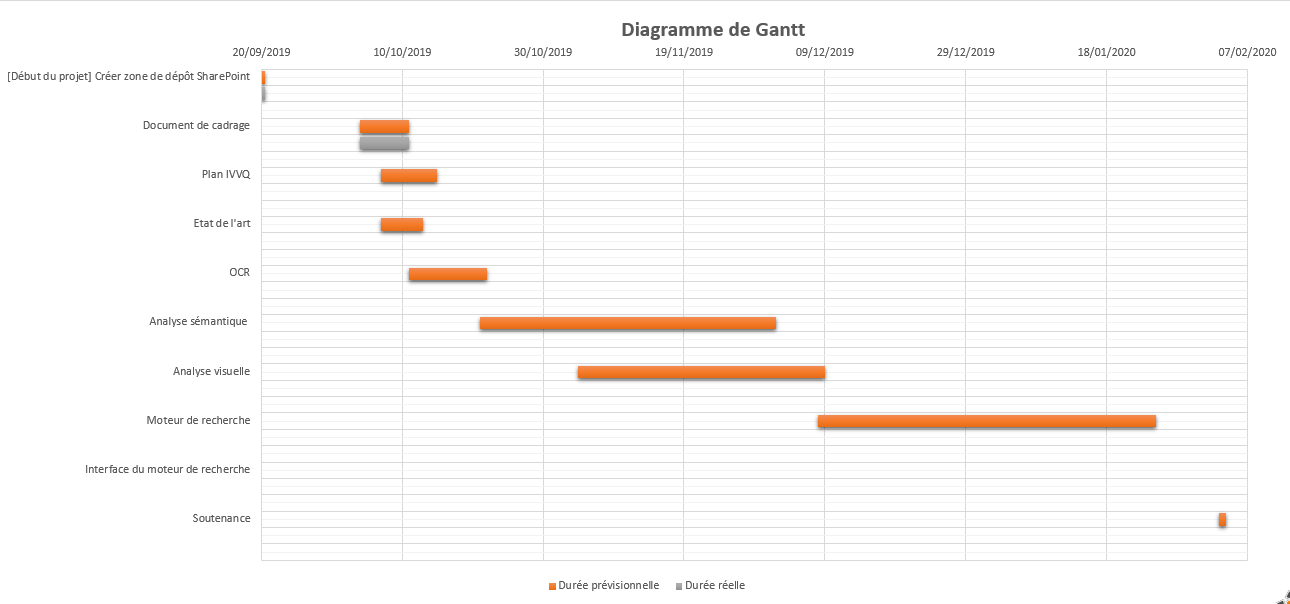
\includegraphics[width=\linewidth]{gantt.png}
	\caption{Diagramme de Gantt prévisionnel}
	\label{fig:ganttprev}
\end{figure}

Le figure~\ref{fig:ganttprev} représente le diagramme de Gantt prévisionnel qui nous a permis de nous aiguiller tout le long du projet.
En orange nous avons la durée des tâches que nous avons estimées et en gris leurs durées réelles.

Voici également le diagramme de Gantt post Mortem (figure~\ref{fig:postmortem}), complété tout au long du projet.
\begin{figure}[h!]
  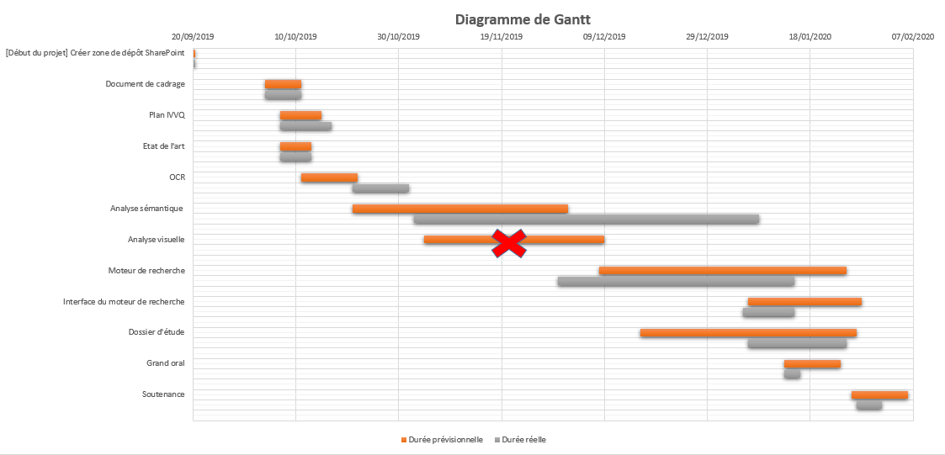
\includegraphics[width=\linewidth]{DiagrammeGanttAvantXL.png}
	\caption{Diagramme de Gantt post moderm}
	\label{fig:postmortem}
\end{figure}


Nous pouvons remarquer que nous sommes généralement dans les temps même si certaines tâches ont pris plus de temps que prévues.
L'analyse sémantique représente la taxonomie qui est la charge de travail la plus importantes. 

L'analyse visuel a été supprimé suite à une réunion avec le commanditaire ou nous avons réduit le cadre du projet pour avoir une chance de le finir.
Cette réduction de cadre a rendu la fonctionnalité de cette tâche inutile.
De ce fait, nous avons gagné plus de temps pour nous focaliser sur d'autres tâches. 


\subsection{Gantt Hebdomadaire}
Le diagramme de Gantt prévisionnel (\ref{fig:ganttprev}) est utile pour contrôler l'avancement du projet.

Cependant, chaque grande tâche est composée de tâches plus petites. 
C'est la raison pour laquelle nous avons fait un diagramme de Gantt hebdomadaire pour chaque sprint d'une semaine.

\begin{figure}[h!]
  \centering
  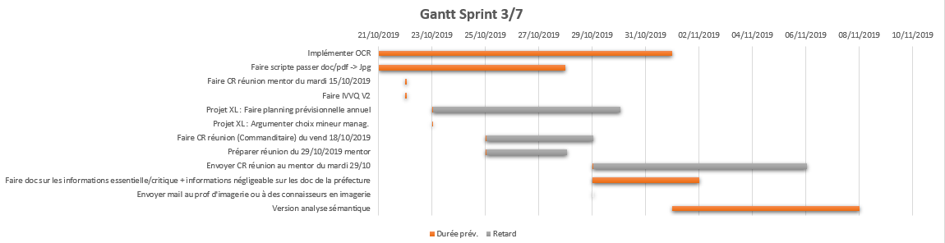
\includegraphics[width=0.8\textwidth]{DiagrammeGanttHebdoAvantXL.png}
  \caption[]{Diagramme de Gantt hebdomadaire sprint 3/7}
  \label{fig:gantthebdo}
\end{figure}

Cette démarche nous a été d’une grande aide pour nous guider sur notre avancement.
La figure~\ref{fig:gantthebdo} nous avons l'exemple du sprint 3/7 qui concerne la demande de projet XL et l'implémentation d'une méthode d'OCR\@. 
Nous avons des indications sur la durée que nous avons prévu (en orange) et le retard que nous avons pris (en gris). 


\subsection{Organisation}
L'équipe du projet est composée de deux étudiants Lavallois et un étudiant Parisiens.
Cette situation géographique n'a pas été un handicap car cela nous a permis d'organiser des réunions régulières avec le commanditaire à la prefecture de la Mayenne, située a Laval. 
Les réunions se sont en grande majorité par visioconférence en utilisant Discord, Facebook et Microsoft Teams en fonction de la situation.

Les membres de l'équipe sur Laval ont également pu effectuer une rencontre avec des archivistes dans le bâtiment des archives départementales.

\subsubsection{Sharepoint et Github}
Afin de gérer nos documents facilement, l'ensemble des fichiers non-techniques ont été placés sur le Sharepoint Cap Projet.
Nous considérons comme non-techniques les documents administratifs, nos comptes rendus de réunions, les recueils administratifs de la préfecture et le trombinoscope.
Nos rapports n'y sont pas stockés car ils ont été rédigés avec \LaTeX, et leur gestion est facilitée par l'utilisation de GitHub.

L'utilisation du SharePoint nous permet également d’informer automatiquement notre mentor lorsqu'un document est disponible. 

En ce qui concerne la gestion de nos programmes, nous avons fait le choix de travailler avec Github qui est un service web d'hébergement et de gestion de développement de logiciels.
L'utilisation de GitHub nous a permis un contrôle de version des codes et de favoriser la collaboration ainsi que la disponibilité des codes. 


\subsubsection{Réunions}
Pour un suivi régulier du projet, nous avons convenus avec notre mentor d'une réunion par semaine.
Cette réunion s'est pour la plupart du temps déroulée par visioconférence en raison de la situation géographique de l'équipe.

Lors de la réunion, nous avons utilisé des PowerPoints pour présenter notre travail (image~\ref{fig::ppt}).
Cette démarche permet de structurer la réunion et rend les informations plus lisibles et présentables. 

\begin{figure}[h!]
  \centering
  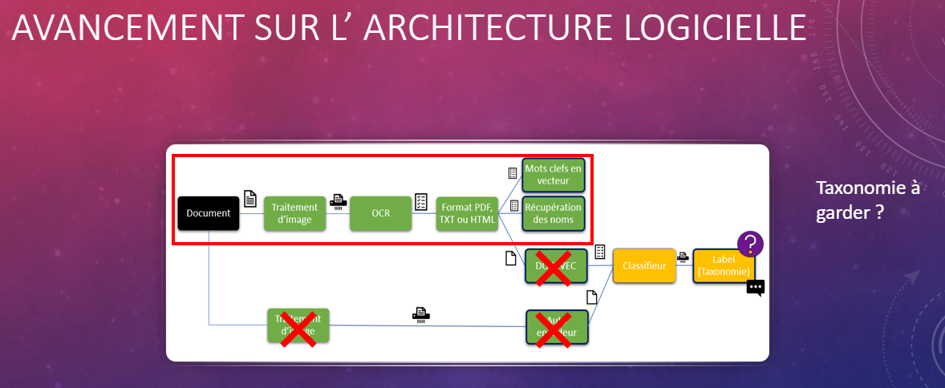
\includegraphics[width=0.8\textwidth]{ArchitecureLogicielAvantXL.png}
  \caption[]{Avancement architecture logiciel}
  \label{fig:ppt}
\end{figure}




\subsection{Charge de travail}
Nous avons commencés par évaluer les charges de travail qui seront nécessaire pour chaque tâche en nous basant sur le Gantt prévisionnel.
Cette démarche nous a permis de réaliser pleinement l'ampleur de ce projet et d'envisager une demande de passage du projet en projet XL\@. 

La charge de travail prévisionnelle est résumée dans la figure~\ref{fig:chargeTravail}.
\begin{figure}[h!]
  \centering
  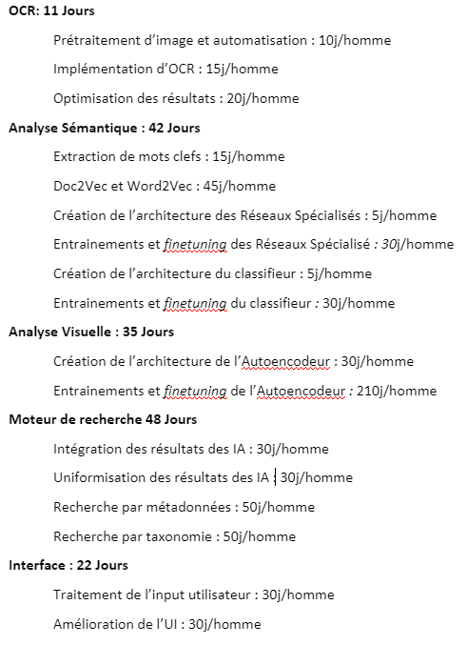
\includegraphics[width=\linewidth]{ChargeDeTravailAvantXL.png}
	\caption[]{Charge de travail prévisionnel}
	\label{fig:chargeTravail}
\end{figure}

Nous avons également prévu une marge sur l'évaluation des tâches en jours/hommes pour prévenir des différents risques que nous pourrions rencontrer.
La charge de travail réel calculée a la fin du projet est un peu moins de deux fois supérieure que ce que nous avions précédaient évalué. 

En réalité, nous avons effectué une charge de travail équivalent à 848 heures.




\section{Durant la période XL}
Suite à l'évaluation des charges de travails, nous avons réalisé une demande de projet XL qui consiste à remplacer la mineures managériale par des heures disponibles pour la réalisation de notre PFE\@.
Cette demande ayant été acceptée, nous avons changé notre approche.
Le projet XL aura duré trois semaines, du 6 janvier 2020 au 25 janvier 2020.

\subsection{Organisation}
Dans un premier temps, nous avons jugé qu'il était nécessaire de revoir notre organisation.
Le nombre de jours disponible étant d'un coup bien plus grand, nous avons redistribué les taches pour couvrir efficacement les jours disponibles.

Nous avons décidé d'appliquer au mieux la méthode agile Scrum pour favoriser le développement et être surs que notre produit conviendrait aux attentes du commanditaire.
Cette méthode a portée ses fruits, le commanditaire étant très satisfait du POC que nous lui avons fourni.

Après avoir listé l'ensemble des tâches, nous les avons divisés en deux sprints:
\begin{itemize}
    \item Sprint 1:\newline
    Version 1 PoC.
    Semaine du 6 janvier au 10 janvier 
    \item Sprint 2:\newline
    Version 2 PoC et DER\@.
    Semaine du 13 janvier au 5 février
\end{itemize}

Le sprint 2 a une durée plus grande que le premier a cause de la différente charge de travail.
Il correspond en partie aux tâches non techniques, comme la rédaction du DER et les préparations du Grand Oral et de la Soutenance. 


\subsection{Trello}
Trello est un outil de gestion de projet en ligne, lancé en septembre 2011 et inspiré par la méthode Kanban de Toyota.
Il repose sur une organisation des projets en planches listant des cartes, chacune représentant une tâche. 

Durant toute la période XL du projet, nous avons utilisé Trello pour visualiser nos taches, leurs états et leurs avancement. 
Pour mieux s’organiser, nous avons divisé les tâches en six parties ayant chacune un code couleur: 

\begin{itemize}
    \item Métadonnées: Bleu ciel 
    \item Taxonomie: Bleu foncé 
    \item Moteur de recherche (JSON et interface): vert
    \item DER\@: Jaune
    \item Grand Oral: Rose
    \item Soutenance: Violet 
\end{itemize}


\begin{figure}[h!]
  \centering
  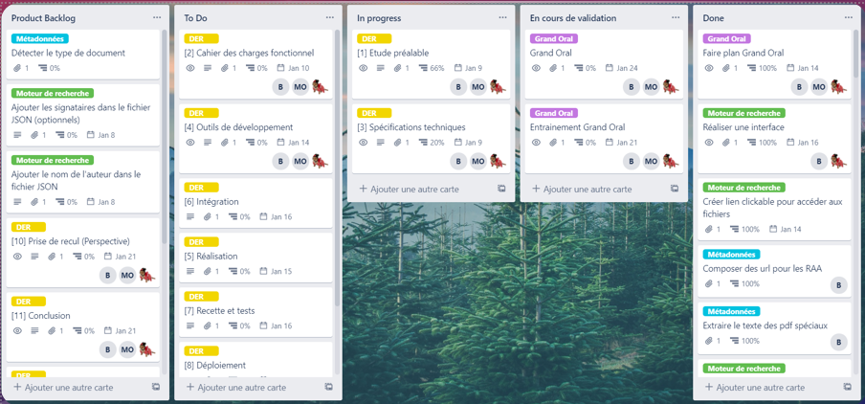
\includegraphics[width=0.8\textwidth]{ScrumBoardXL.png}
	\caption[]{Scrum board dans Trello}
	\label{fig:trello}
\end{figure}

Ce tableau de bord du projet (figure~\ref{fig:trello}) est accessible en ligne et visible en permanence pour notre équipe.
Il permet de suivre en temps réel l'évolution des tâches et des user stories à réaliser.

Le scrum board est séparé au minimum en quatre parties: Le product backlog, les tâches à faire, les tâches en cours et les tâches terminées.
Nous avons ajouté une phase `En cours de validation' afin de vérifier que les tâches ont bien été faite. 
Cette validation est réalisée par le Product Owner.

L'utilisation de Trello a grandement facilité notre organisation.
Tous les jours, lors de la première réunion, nous décidions ensemble des tâches de la journée graphiquement.
Nous pouvions alors mettre a jour nos tâches et leurs avancements en temps réel au long de la journée.

\subsection{Scrum}
La méthode agile permet de délivrer un projet/produit très rapidement.
Ce cadre méthodologique est conçu sur des cycles de développement court durant lesquels on s'adapte constamment tout en maintenant l'utilisateur au centre. 

Pour fonctionner, elle a besoin de plusieurs rôles:
\begin{itemize}
    \item \textbf{Scrum master}\newline
    Le scrum master est garant du processus scrum.
    Il s'assure d’une bonne communication entre les membres de l'équipe.
    Afin que l'équipe comprenne bien cette méthodologie de travaille, le scrum master a écrit un document qui l'explique en détail.

    \item \textbf{Product Owner}\newline
    Le Product Owner représente le client.
    Il définit les spécifications fonctionnels (exemple:  document Integration Validation Verification Qualification) et établie la liste des priorités de ce qu'il faut développer.
    C'est aussi lui qui valide les fonctionnalités.
    

    \item \textbf{Développeurs}\newline
    Ici, les développeurs sont tous les agents techniques du projet.
\end{itemize}

\subsubsection{User Story}
Le processus Scrum commence par l'écriture d'une user story.
Cette User Story décrit l'expérience utilisateur en utilisant le langage, le vocabulaire et la terminologie de l'usager.   

Chaque user story comporte: 
\begin{itemize}
    \item \textbf{Un identifiant}: un nom contenant la fonction du produit de manière succincte  
    \item \textbf{L'importance}: Une valeur qui définit la priorité de la story  
    \item \textbf{Estimation} du travail nécessaire
    \item \textbf{Démonstration}: Un test simple de la story qui sera à valider   
\end{itemize}

L'image~\ref{fig:userStory} montre un exemple d'une des User Story que nous avons défini.
\begin{figure}[h!]
  \centering
  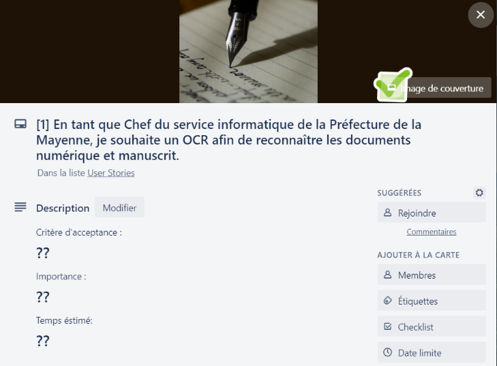
\includegraphics[width=0.8\textwidth]{userStoryXL.png}
	\caption[]{Exemple d’un user story}
	\label{fig:userStory}
\end{figure}

Cette étape nous a permis de nous recontextualiser le PoC demandé par le commanditaire. 


\subsubsection{Product backlog}
De la User Story va émaner des exigences.
Elles seront hiérarchisées avec le client dans un product backlog que nous pouvons voir comme un carnet de commande. 
C'est un miroir de ce qu'il faut faire pour réaliser les besoins du client.  

Le product backlog va constamment évoluer pour refléter les nouveaux besoins du client (après un sprint). 
La liste prévisionnelle des tâches définie est visible dans l'image~\ref{fig:listeTaches}, ainsi que le product backlog généré avec Trello sur l'image~\ref{fig:prodBack}.

\begin{figure}
  \centering

  \begin{subfigure}{.5\textwidth}
    \centering
    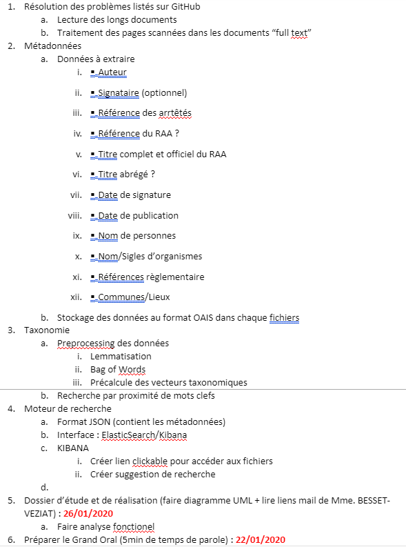
\includegraphics[width=\linewidth]{ListePrevisionnelleXL.png}
    \caption[]{Liste prévisionnelle des taches}
    \label{fig:listeTaches}
  \end{subfigure}%
  \begin{subfigure}{.5\textwidth}
    \centering
    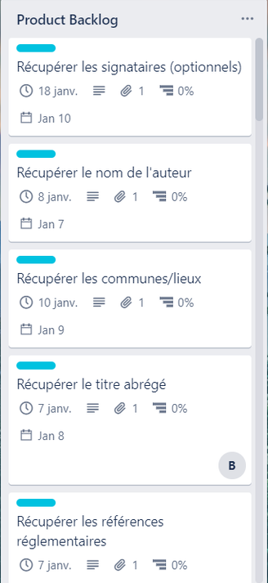
\includegraphics[width=0.6\linewidth]{ProductBacklogXL.png}
    \caption[]{Product backlog avec Trello}
    \label{fig:prodBack}
  \end{subfigure}

\end{figure}

\subsubsection{Sprint}
Une fois la user story et les exigences (product backlog) fixés, nous pouvons nous lancer dans la réalisation.
La réalisation sera découpée en plusieurs itérations que l'on nomme des sprints. 

Les étapes du sprint sont:
\begin{itemize}
    \item \textbf{Sprint planning meeting}

    Un sprint commence par une réunion de planification.
    Au cours de cette séance, on va aller puiser les éléments prioritaires du product backlog qui seront développés dans les sprints.
    Aussi nommé daily meeting, nous avons utilisé cette méthode.
    Nous avons effectué une réunion tous les matins à 10h du lundi au vendredi afin d'attribuer les tâches de la journée.
    Nous avons rajouté une autre réunion le soir à partir de 19h qui n’est pas prévu dans la méthode Scrum.
    Cette dernière réunion nous a permis de revoir les difficultés que nous avons rencontré et de discuter des tâches effectuées dans la journée. 

    \item \textbf{Sprint backlog}

    Dans chaque sprint, qui durent entre une et deux semaines, il y aura du développement puis un contrôle qualité (des tests) et une livraison.
    L'ensemble des livraisons des sprints cumulés se nomment le sprint backlog.
\end{itemize}



\subsection{Horaires}
Nos horaires de travails étaient en moyenne de 10h à 18h avec une pause déjeuner vers 12h.
Nous avions une réunion tous les matins à 10h et une le soir vers 19h.



\subsection{Charge de travail}

En listant l'ensemble de tâches, nous avons établi leurs charges de travail en jours/hommes et en heures. 
Voici les tâches et leurs durées prévisionnelles et réelles.

\textbf{Prévisionnel} 
\begin{itemize}
    \item Sprint 1 (6 janvier au 10 janvier):
        \begin{itemize}
            \item Métadonnées: 6 jours/hommes pour 2 personnes
            \item Taxonomie: 18 jours/hommes pour 1 personnes
            \item Moteur de recherche: 15 jours/hommes 2 personnes
        \end{itemize}
    \item Sprint 2 (13 janvier au 3 février):
    \begin{itemize}
        \item DER\@: 11 jours/hommes pour 3 personnes
        \item Grand Oral: 6 jours/hommes pour 3 personnes
        \item Soutenance:  9 jours/hommes pour 3 personnes
    \end{itemize}
\end{itemize} 

Nous avions estimé un total de 65 jours/hommes de travail en 3 semaines pour 3 personnes.


\textbf{Réel}

\begin{itemize}
    \item Sprint 1 (6 janvier au 10 janvier):
        \begin{itemize}
            \item Métadonnées: 9 jours/hommes pour 2 personnes
            \item Taxonomie: 12 jours/hommes pour 1 personnes
            \item Moteur de recherche: 31 jours/hommes 2 personnes
        \end{itemize}
    \item Sprint 2 (13 janvier au 3 février):
    \begin{itemize}
        \item DER\@: 18 jours/hommes pour 3 personnes
        \item Grand Oral: 8 jours/hommes pour 3 personnes
        \item Soutenance:  9 jours/hommes pour 3 personnes
    \end{itemize}
\end{itemize} 

Nous avons effectué un total de 127 jours/hommes en 3 semaines pour 3 personnes.

Sur la figure~\ref{fig:chargeReel}, nous pouvons voir la comparaison des charges de travail réel contre ce que nous avions prévu en jours/hommes.

\begin{figure}[h!]
  \centering
  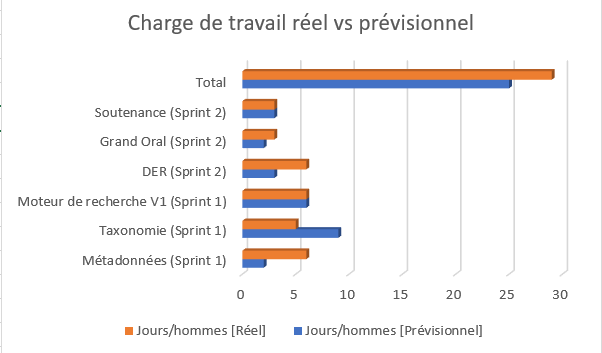
\includegraphics[width=0.6\textwidth]{ChargeTravailXL.png}
	\caption[]{Charge de travail prévisionnel contre réel en jours/hommes}
	\label{fig:chargeReel}
\end{figure}



\subsection{Gantt prévisionnel/réel}
Au début du projet XL, nous avons réalisé un diagramme de Gantt prévisionnel afin de comparer les charges de travails ainsi que la durée de chacune des taches.
Le diagramme du projet XL commence le 6 janvier 2020 et se termine le 5 février 2020. 

Sur les images~\ref{fig:gantXLprev} et~\ref{fig:gantXLreel}, nous avons également listé certaines taches datant du 2 décembre pour montrer les dépendances qu'elles provoquent.
De plus, on peut remarquer que nous avons des indications de pourcentage de completion pour le projet et les taches.

Dans notre Trello, lorsqu'une tâche est dans le product backlog ou dans la section `To do' elle est automatiquement à 0\%.
En passant dans `In progress' elle passe à 20\%, dans `En cours de validation' à 80\% puis à 100\% lorsqu'elle est dans `Done'.
Nous obtenons ainsi un diagramme dynamique avec une métrique plus intéressante comparé à notre ancien Gantt, assez fixe.

\begin{figure}
   \centering
   \begin{subfigure}{.5\textwidth}
     \centering
     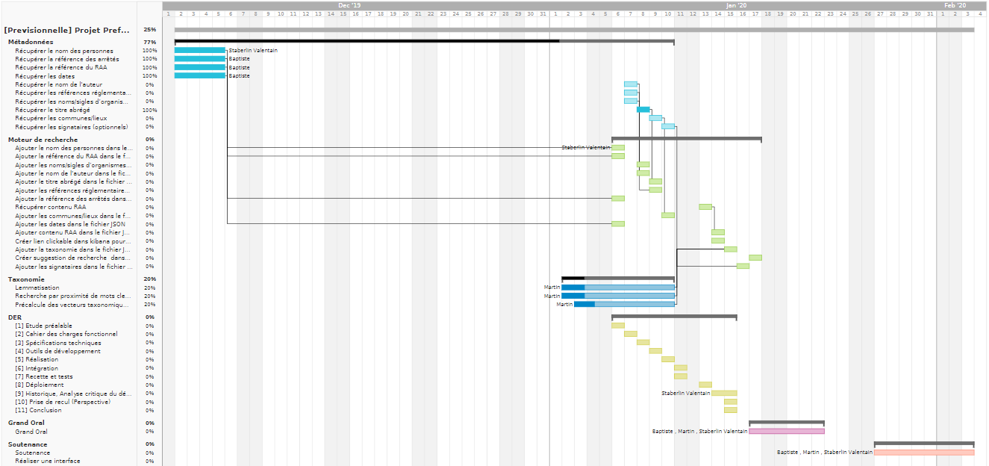
\includegraphics[width=\textwidth]{GanttPrevisionnelXL.png}
   	\caption{Diagramme de Gantt prévisionnel}
   	\label{fig:gantXLprev}
   \end{subfigure}%
   \begin{subfigure}{.5\textwidth}
     \centering
     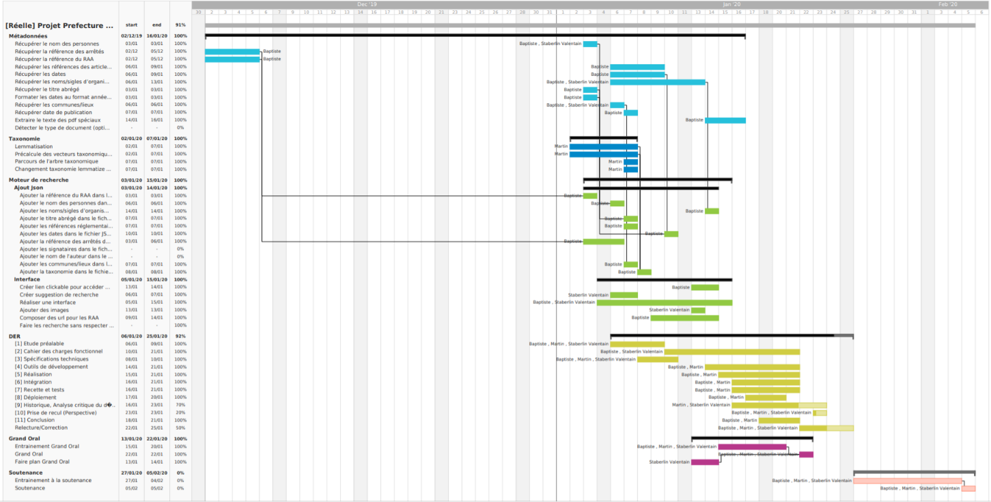
\includegraphics[width=\textwidth]{GanttReelXL.png}
   	\caption{Diagramme de Gantt réel}
   	\label{fig:gantXLreel}
   \end{subfigure}
   \caption{Diagrammes de Gantt Projet XL}
\end{figure}

\subsubsection{Sprint 1: Durée Réel/prévisionnel}
A l'aide de Trello, nous avions établi un calendrier hebdomadaire pour chaque sprint.
Ce dernier nous a permis d’avoir une indication visuelle sur le nombre de tâches par jours que nous devons prévoir, réaliser et valider.
Si nous devions comparer l'image~\ref{fig:gantPrevHebdo1} et l'image~\ref{fig:GantReelHebdo1} (Gantt prévisionnel et réel), nous pouvons remarquer que certaines tâches ont pris moins de temps que prévu, mais que la quantité de travails par jours est plus importante dans la réalité.

\begin{figure}
   \centering
   \begin{subfigure}{.5\textwidth}
     \centering
     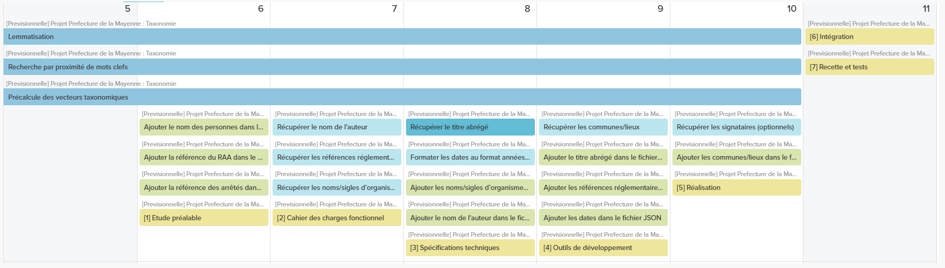
\includegraphics[width=\textwidth]{GanttPrevHebdoSprint1XL.png}
   	\caption[]{Calendrier prévisionnel}
   	\label{fig:gantPrevHebdo1}
   \end{subfigure}%
   \begin{subfigure}{.5\textwidth}
     \centering
     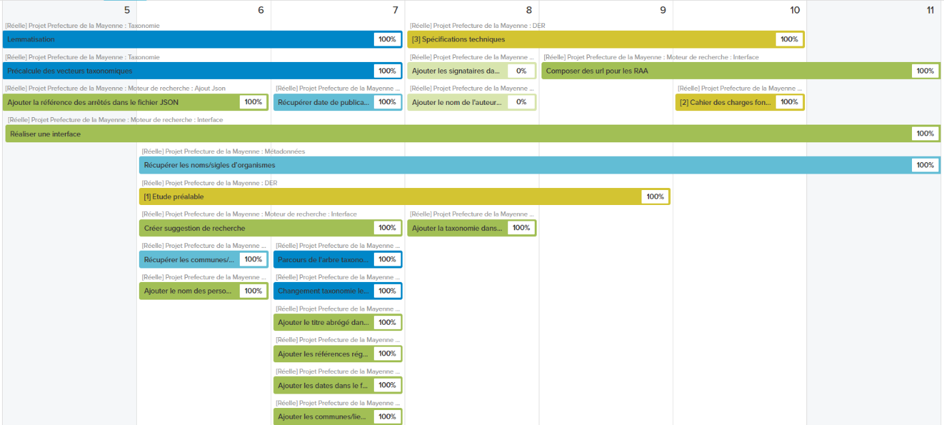
\includegraphics[width=\textwidth]{GanttReelHebdoSprint1XL.png}
   	\caption[]{Calendrier réel}
   	\label{fig:GantReelHebdo1}
   \end{subfigure}
   \caption{Calendrier Sprint 1}
\end{figure}


\subsubsection{Sprint 2: Durée Réel/prévisionnel}
Le deuxième sprint est plutôt consacré au DER, au Grand Oral ainsi qu'à la soutenance.
Nous n'avons pas prévu que le DER aurait pris autant de temps (visible sur les images~\ref{fig:gantPrevHebdo2} et~\ref{fig:GantReelHebdo2}).
Comme résultat, nous nous sommes retrouvés a effectué plus de tâches que prévues par jours. 

\begin{figure}
  \centering
  \begin{subfigure}{.5\textwidth}
    \centering
    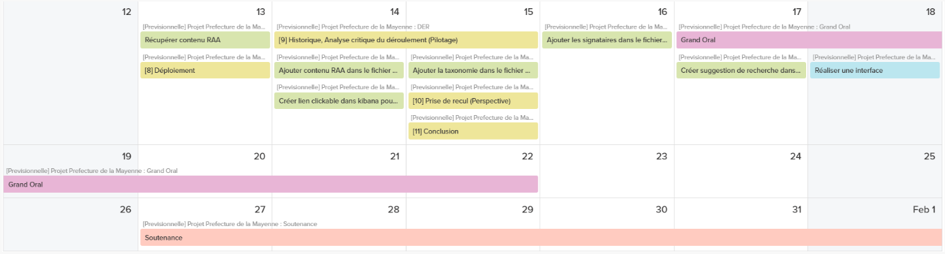
\includegraphics[width=\textwidth]{GanttPrevHebdoSprint2XL.png}
  	\caption[]{Calendrier prévisionnel Sprint 2}
  	\label{fig:gantPrevHebdo2}
  \end{subfigure}%
  \begin{subfigure}{.5\textwidth}
    \centering
    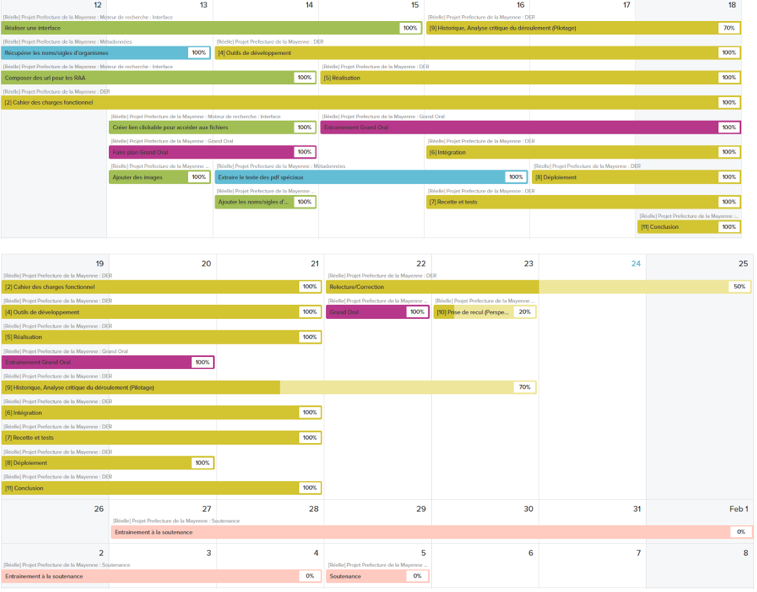
\includegraphics[width=\textwidth]{GanttReelHebdoSprint2XL.png}
  	\caption[]{Calendrier réel Sprint 2}
  	\label{fig:GantReelHebdo2}
  \end{subfigure}
\end{figure}

Même si le diagramme de Gantt n'a pas été respecté tel que prévu, le fait d’avoir estimé les charges de travails ainsi que d'établir un calendrier de travail cela nous a permis d'être à temps sur l'ensemble du projet.
Nous pouvons en déduire que la méthode agile a accéléré l'avancement du projet.








